%\clearpage
\chapter{Systems modelled by differential equations}\label{sec:syst-modell-diff}

\begin{figure}[tp]
\centering
\begin{circuitikz} \draw
 %(0,0) node[anchor=east]{B}
  (0,0) to[short, o-*] (3,0)
  to[C, l=$C$, *-*] (3,3)
  (3,3) to[R, l=$R$, *-o] (0,3)
  to[open, v=$x(t)$] (0,0)
  (3,0) to[short, *-o] +(1,0)
  to[open,v_>=$y(t)$, -o] +(0,3)
  (4,3) to[short, -*] (3,3)
;\end{circuitikz}
\caption{An electrical circuit with resistor and capacitor in series, otherwise known as an \term{RC circuit}.} \label{circ:seriesRC1}
\end{figure}


\begin{figure}[tp]
\centering
\begin{tikzpicture}
\tikzstyle{spring}=[thick,decorate,decoration={coil,pre length=0.3cm,post length=0.3cm,segment length=6,aspect=0.9}]
\tikzstyle{damper}=[thick,decoration={markings,  
  mark connection node=dmp,
  mark=at position 0.5 with 
  {
    \node (dmp) [thick,inner sep=0pt,transform shape,rotate=-90,minimum width=15pt,minimum height=3pt,draw=none] {};
    \draw [thick] ($(dmp.north east)+(2pt,0)$) -- (dmp.south east) -- (dmp.south west) -- ($(dmp.north west)+(2pt,0)$);
    \draw [thick] ($(dmp.north)+(0,-5pt)$) -- ($(dmp.north)+(0,5pt)$);
  }
}, decorate]
\tikzstyle{ground}=[fill,pattern=north east lines,draw=none,minimum width=0.75cm,minimum height=0.3cm]

\node (M) [minimum width=3.5cm,minimum height=1.5cm,style={draw,outer sep=0pt,thick}] {mass $M$};

\node (ground1) at (M.north) [ground,yshift=2.5cm,xshift=-1cm,anchor=north] {};
\draw (ground1.south west) -- (ground1.south east);
\draw [spring] (ground1.south) -- ($(M.north east)!(ground1.south)!(M.north west)$) node[pos=.5,left,minimum width=20pt] {$K$};

\node (ground3) at (M.north) [ground,yshift=2.5cm,xshift=1cm,anchor=north] {};
\draw (ground3.south west) -- (ground3.south east);
\draw [damper] (ground3.south) -- ($(M.north east)!(ground3.south)!(M.north west)$) node[pos=.5,right,minimum width=30pt] {$B$};

\draw [latex-,thick] (M.east) ++(0.5cm,-0.5cm) -- +(0cm,1.0cm) node[pos=0.5,right] {$p(t)$};
\draw [latex-,thick] (M.west) ++(-0.5cm,-0.5cm) -- +(0cm,1.0cm) node[pos=0.5,left] {$f(t)$};

% \begin{scope}[xshift=7cm]
% \node (M) [minimum width=1cm, minimum height=2.5cm] {$m$};

% \node (ground) [ground,anchor=north,yshift=-0.25cm,minimum width=1.5cm] at (M.south) {};
% \draw (ground.north east) -- (ground.north west);
% \draw [thick] (M.south west) ++ (0.2cm,-0.125cm) circle (0.125cm)  (M.south east) ++ (-0.2cm,-0.125cm) circle (0.125cm);

% \node (wall) [ground, rotate=-90, minimum width=3cm,yshift=-3cm] {};
% \draw (wall.north east) -- (wall.north west);

% \draw [spring] (wall.170) -- ($(M.north west)!(wall.170)!(M.south west)$);
% \draw [damper] (wall.10) -- ($(M.north west)!(wall.10)!(M.south west)$);

% \draw [-latex,ultra thick] (M.east) ++ (0.2cm,0) -- +(1cm,0);
% \end{scope}
\end{tikzpicture}
\caption{A mechanical mass-spring-damper system} \label{mech:massspring1}
\end{figure}


%Let $H$ be a system and let $y = H(x)$ be the response of the system to input signal $x$.  
Systems of particular interest in this text are those where the input signal $x$ and output signal $y$ are related by a linear differential equation with constant coefficients, that is, an equation of the form
\[
\sum_{\ell=0}^{m} a_\ell \frac{d^\ell}{d t^\ell} x(t) = \sum_{\ell=0}^{k} b_\ell \frac{d^\ell}{d t^\ell} y(t),
\]
where $a_0,\dots,a_m$ and $b_0,\dots,b_k$ are real or complex numbers.  In what follows we use the differentiator system $D$ rather than the notation $\frac{d}{d t}$ to represent differentiation.  To represent the $\ell$th derivative we write $D^\ell$ instead of  $\frac{d^\ell}{d t^\ell}$.  Using this notation the differential equation above is
\begin{equation}\label{eq:diffequform}
\sum_{\ell=0}^{m} a_\ell D^\ell(x) = \sum_{\ell=0}^{k} b_\ell D^\ell(y). 
\end{equation}
%To keep the notation clean we do not usually write the argument $(t)$ for a signal $x$.

Equations of this form can be used to model a large number of electrical, mechanical and other real world devices.  For example, consider the resistor and capacitor (RC) circuit in Figure~\ref{circ:seriesRC1}.  Let the signal $v_R$ represent the voltage over the resistor and $i$ the current through both resistor and capacitor.  The voltage signals satisfy
\[
x = y + v_R,
\]
and the current satisfies both
\[
v_R = R i \qquad \text{and} \qquad i = C D(y).
\]
Combining these equations,
\begin{equation}\label{eq:RCdiffeq}
x = y + RC D(y)
\end{equation}
that is in the form of~\eqref{eq:diffequform}.

As another example, consider the mass-spring-damper in Figure~\ref{mech:massspring1}.  A force represented by the signal $f$ is externally applied to the mass, and the position of the mass is represented by the signal $p$.  The spring exerts force $-K p$ that is proportional to the position of the mass, and the damper exerts force $-B D(p)$ that is proportional to the velocity of the mass.  The cumulative force exerted on the mass is
\[
f_m = f - K p - B D(p)
\]
and by Newton's law the acceleration of the mass $D^2(p)$ satisfies
\[
M D^2(p) = f_m = f - K p - B D(p).
\]
We obtain the differential equation
\begin{equation}\label{eq:diffeqmasspringdamper}
f = K p + B D(p) + M D^2(p)
\end{equation}
that is in the form of~\eqref{eq:diffequform} if we put $x = f$ and $y = p$.   Given $p$ we can readily solve for the corresponding force $f$.  As a concrete example, let the spring constant, damping constant and mass be $K=B=M=1$.  If the position satisfies $p(t) = e^{-t^2}$, then the corresponding force satisfies
\[
f(t) = e^{-t^2} (4 t^2-2 t-1).
\]
Figure~\ref{fig:masspringdampersol1} depicts these signals.

What happens if a particular force signal $f$ is applied to the mass?  For example, say we apply the force
\[
f(t) = \Pi(t - \tfrac{1}{2}) = \begin{cases}
1 & 0 < t \leq 1 \\
0 & \text{otherwise}.
\end{cases}
\]
What is the corresponding position signal $p$?  We are not yet ready to answer this question, but will be later (Exercise~\ref{exer:massspringdamperrect}).  % We posed this question and others in Section~\ref{sec:syst-modell-diff}.  Imagine we could find a system $H^{-1}$ that \emph{inverts} $H$.  That is, a system $H^{-1}$ with the property
% \[
% x = T_0(x) = H^{-1}\big( H(x) \big).
% \]
% Given $H^{-1}$ we could then find $p$ by applying $H^{-1}$ to $f$ because
% \[
% p = H^{-1}\big(H(p)\big) = H^{-1}(f). 
% \]
% Does an inverse system $H^{-1}$ exists? If so, how do we find it?  It turns out that in many cases of pratical interest, inverses of linear time-invariant systems do exist, and that the inverses themselves are linear and time-invariant.  Developing techniques for finding inverse systems is left until we introduce the Laplace transform in Section~\ref{sec:laplace-transform}.

\begin{figure}[tp]
\centering
\defaultanimation{tikzfigs/masspringdampersolution}
%\animategraphics[autoplay,loop,every=\every]{\defaultframerate}{tikzfigs/masspringdampersolution}{}{}
\caption{A solution to the mass-spring-damper system with $K=B=M=1$.  The position is $p(t) = e^{-t^2}$ with corresponding force $f(t) = e^{-t^2} (4 t^2-2 t-1)$.} \label{fig:masspringdampersol1}
\end{figure}

In both the mechanical mass-spring-damper system in Figure~\ref{mech:massspring1} and the electrical RC circuit in Figure~\ref{circ:seriesRC1} we obtain a differential equation relating the input signal $x$ with the output signal $y$.  The equations do not specify the output signal $y$ explicitly in terms of the input signal $x$, that is, they do not explicitly define a system $H$ such $y = H(x)$.  As they are, the differential equations do not provide as much information about the behaviour of the system as we would like.  For example, is the system stable?
%Is it invertible?  
We will be able to obtain much more information about these systems when the \term{Laplace transform} is introduced in Chapter~\ref{sec:laplace-transform}.
%The , described , is a useful tool for obtaining more information about these systems.  %A key property enabling the Laplace transform is that differential equations of the form~\eqref{eq:diffequform} describe systems that are linear and time-invariant.% (Exercise~\ref{excer:differeqarelti}).  %To see this let $x_1$, $y_1$ and $x_2$,$y_2$ be solutions of an equation in the form~\eqref{eq:diffequform}.  For any real numbers $c$ and $d$,
% \[
% c \sum_{\ell=0}^{m} a_\ell D^\ell(x_1) = c \sum_{\ell=0}^{k} b_\ell D^\ell(y_1)
% \]
% and 
% \[
% c \sum_{\ell=0}^{m} a_\ell D^\ell(x_1) = c \sum_{\ell=0}^{k} b_\ell D^\ell(y_1)
% \]
%We further study linear, time-invariant systems in Section~\ref{sec:prop-line-time}.  
The remainder of this chapter details the construction of differential equations that model various mechanical, electrical, and electro-mechanical systems.  We will use the systems constructed here as examples throughout the course.

\section{Passive electrical circuits}

\term{Passive electrical circuits} require no sources of power other than the input signal itself.  For example, the voltage divider in Figure~\ref{circ:voltagedivider} and the RC circuit in Figure~\ref{circ:seriesRC1} are passive circuits.  Another common passive electrical circuit is the resistor, capacitor and inductor (RLC) circuit depicted in Figure~\ref{circ:seriesRLC1}.  In this circuit we let the output signal $y$ be the voltage over the resistor.  Let $v_C$ represent the voltage over the capacitor and $v_L$ the voltage over the inductor and let $i$ be the current.  
We have
\[
y = Ri, \qquad i = C D(v_C), \qquad v_L = L D(i),
\]
leading to the following relationships between $y$, $v_C$ and $v_L$,
\[
y = R C D(v_C), \qquad R v_L = L D(y).
\]
Kirchhoff's voltage law gives $x = y + v_C + v_L$ and by differentiating both sides
\[
D(x) = D(y) + D(v_C) + D(v_L).
\]
Substituting the equations relating $y$, $v_C$ and $v_L$ leads to
\begin{equation}\label{eq:RLCdiffeq}
RC D(x) = y+ RC D(y) + LC D^2(y).
\end{equation}
We can similarly find equations relating the input voltage with $v_C$ and $v_L$.

\begin{figure}[tp]
\centering
\begin{circuitikz} \draw
 %(0,0) node[anchor=east]{B}
  (0,0) to[L, l=$L$, o-*] (3,0)
  to[R, l=$R$, *-*] (3,3)
  (3,3) to[C, l=$C$, *-o] (0,3)
  to[open, v=$x(t)$] (0,0)
  (3,0) to[short, *-o] +(1,0)
  to[open,v_>=$y(t)$, -o] +(0,3)
  (4,3) to[short, -*] (3,3)
;\end{circuitikz}
\caption{An electrical circuit with resistor, capacitor and inductor in series, otherwise known as an \term{RLC circuit}.} \label{circ:seriesRLC1}
\end{figure}

% We will now test the properties of this circuit.

% \begin{test}\label{test:rlctest1}
% \emph{
% In this test we construct the RLC circuit from Figure~\ref{circ:seriesRLC1} on a breadboard with restance $R=?$, capacitance $C=?$ and inductance $L=?$.  Using a computer soundcard (an approximation of) the voltage signal
% \[
% x(t) = \sin( 2 \pi f_1 t) + \sin( 2\pi f_2 t) + \tfrac{2}{3}\sin( 2\pi f_3 t)
% \]
% with $f_1 = 400, f_2 = 1000, f_3 = 3000$ is passed through the circuit.  As in previous tests, the soundcard is used to sample the input signal and the output signal, in this case the voltage over the resistor. Approximate reconstructions of the input signal $\tilde{x}$ and output signal $\tilde{y}$ are given according to~\eqref{eq:xreconstruct}, and~\eqref{eq:yreconstruct}.  According to~\eqref{eq:RLCdiffeq} we expect the approximate relationship
% \[
% RC D(\tilde{x}) \approx \tilde{y} + RC D(\tilde{y}) + LC D^2(\tilde{y}).
% \]
% The derivative of the sinc function is given in~\eqref{eq:sincderivative} and the second derivative is
% \[
% D^2(\sinc,t) = \frac{1}{\pi  x^3}\big( (2-\pi ^2x^2)\sin(\pi x) -2 \pi  x\cos(\pi  x) \big).
% \]
% Similarly to~\eqref{eq:Dtildey}, the $k$th derivatives of $\tilde{x}$ and $\tilde{y}$ are
% \[
% D^k(\tilde{y}) = \sum_{\ell=1}^L y_\ell D^k(\sinc, t - F\ell),
% \]
% \[
% D^k(\tilde{x}) = \sum_{\ell=1}^L x_\ell D^k(\sinc, t - F\ell).
% \]
% }
% \end{test}


% \begin{test}\label{test:rctest1}
% (\textbf{RC circuit})
% In this test we construct an RC circuit on a breadboard with restance $R=22\kilo\si{\ohm}$ and capacitance $C=47\micro\farad$.  Using a computer soundcard (an approximation of) the voltage signal
% \[
% x(t) = \sin( 2 \pi f_1 t) + \sin( 2\pi f_2 t)
% \]
% with $f_1 = 100$ and $f_2 = 133$ is passed through the circuit.  The approximation is generated by sampling $x(t)$ at rate $F = \frac{1}{T_s} = 44100$ to generate the samples $x_n = x(n T_s) \qquad n = 0, \dots, 2 F$ that are passed to the sound card.  The voltage over the capacitor is recorded returning a list of samples $y_1,\dots,y_L$ taken at rate $F$.  The input voltage is simultaneously recorded into a list of samples $x_1,\dots,x_L$.  As in Test~\ref{test:voltagedividertest1}, an approximate reconstruction of the input voltage signal $\tilde{x}$ is given according to~\eqref{eq:xreconstruct}, and an approximate recontruction of the voltage over the capacitor $\tilde{y}$ is given according to~\eqref{eq:yreconstruct}.  According to~\eqref{eq:RCdiffeq} we expect the approximate relationship
% \[
% \tilde{x} \approx \tilde{y} + RC D(\tilde{y}).
% \]
% The derivative of the sinc function is
% \begin{equation}\label{eq:sincderivative}
% D(\sinc,t) = \frac{1}{\pi t^2} \big( \pi t \cos(\pi t) - \sin(\pi t) \big),
% \end{equation}
% and
% \begin{equation}\label{eq:Dtildey}
% D(\tilde{y}) = D\left(\sum_{\ell=1}^L y_\ell \sinc(t - F\ell) \right) = \sum_{\ell=1}^L y_\ell D(\sinc, t - F\ell)
% \end{equation}
% because $D$ is linear and time invariant.  % The approximate relationship can be written $\tilde{x} \approx H(\tilde{y})$ where
% % \begin{equation}\label{eq:Htest:rctest1}
% % H(\tilde{y}) = \tilde{y} + RC \sum_{\ell=1}^L y_\ell D(\sinc, t - F\ell)
% % \end{equation}
% \end{test}

% \begin{figure}[tp]
% \includegraphics{tests/rc/plot-1.mps}
% \caption{Plot of recieved samples of voltage over the capacitor of an RC circuit}\label{fig:test1:RCplotrecievedsamples}
% \end{figure}


\section{Active electrical circuits}\label{sec:active-circuits}

\begin{figure}
\centering
\begin{circuitikz}
\node[op amp,yscale=-1.3,xscale=1.3] (oa) {};
\draw (oa.+) to[short,o-] (oa.+);
\draw (oa.-) to[short,o-] (oa.-);
\draw (oa.out) to[short,o-] (oa.out);
\node[left] at (oa.+) {$v_{+}$};
\node[left] at (oa.-) {$v_{-}$};
\draw (oa.up) to[short,-o] ++(0,-0.5)
to[open,l_=$v_{--}$] ++(0,0);
\draw (oa.down) to[short,-o] ++(0,0.5) 
to[open,l_=$v_{++}$] ++(0,0);
\node[right] at (oa.out) {$v_{o}$};
\end{circuitikz}  
\qquad
\begin{circuitikz}
\node[left] at (-1,-2) {$v_{-}$};
\node[left] at (-1,0) {$v_{+}$};
\draw (-1,-2) to[short, o-] (0,-2)
to[R,l=$R_i$] (0,0)
to[short,-o] ++(-1,0);
\draw (1,-2) to[american controlled voltage source,l_=$A(v_{+} - v_{-})$] (1,0)
to[R,l=$R_o$,-o] (3.5,0);
\node[ground] at (1,-2) {};
\node[right] at (3.5,0) {$v_o$};
\end{circuitikz}
\caption{Left: triangular component diagram of an \term{operational amplifier}.  The $v_{++}$ and $v_{--}$ connectors indicate where an external voltage source can be connected to the amplifier.  These connectors will usually be omitted.  Right: model for an operational amplifier including input resistance $R_i$, output resistance $R_o$, and open loop gain $A$.  The diamond shaped component is a dependent voltage source.  This model is usually only useful when the operational amplifier is in a negative feedback circuit.}\label{circ:opamp}
\end{figure}

Unlike passive electrical circuits, an \term{active electrical circuit} requires a source of power external to the input signal.  Active circuits can be modelled and constructed using \term{operational amplifiers} as depicted in Figure~\ref{circ:opamp}.  The left hand side of Figure~\ref{circ:opamp} shows a triangular circuit diagram for an operational amplifier, and the right hand side of Figure~\ref{circ:opamp} shows a circuit that can be used to model the behaviour of the amplifier.  The $v_{++}$ and $v_{--}$ connectors indicate where an external voltage source can be connected to the amplifier.  These connectors will usually be omitted.  The diamond shaped component is a dependent voltage source with voltage $A(v_+ - v_-)$ that depends on the difference between the voltage at the \term{non-inverting input} $v_+$ and the voltage at the \term{inverting input} $v_-$.  The dimensionless constant $A$ is called the \term{open loop gain}.  Most operational amplifiers have large open loop gain $A$, large \term{input resistance} $R_i$ and small \term{output resistance} $R_o$.  As we will see, it can be convenient to consider the behaviour as $A\to\infty$, $R_i\to\infty$ and $R_0\to 0$, resulting in an \term{ideal operational amplifier}.

As an example, an operational amplifier configured as a \term{multiplier} is depicted in Figure~\ref{elec:opampinvertingamplifier}.  This circuit is an example of an operational amplifier configured with \term{negative feedback}, meaning that the output of the amplifier is connected (in this case by a resistor) to the inverting input $v_{-}$.  The horizontal wire at the bottom of the plot is considered to be ground (zero volts) and is connected to the negative terminal of the dependent voltage source of the operational amplifier depicted in Figure~\ref{circ:opamp}.  An equivalent circuit for the multiplier using the model in Figure~\ref{circ:opamp} is shown in Figure~\ref{circ:opampinvertingamplifierequivalent}.  Solving this circuit (Exercise~\ref{exer:multiplieropampwithmodel}) yields the following relationship between the input voltage signal $x$ and the output voltage signal $y$,
\begin{equation} \label{eq:intertingopampmodel}
y = \frac{R_i (R_o - A R_2) }{R_i (R_2+R_o)+R_1 (R_2+R_i + A R_i+R_o)}x.
\end{equation}
For an ideal operational amplifier we let $A\to\infty$, $R_i\to\infty$ and $R_o\to 0$.  In this case terms involving the product $A R_i$ dominate and we are left with the simpler equation
\begin{equation}\label{eq:opampmultipleieridealreponse}
y = -\frac{R_2}{R_1} x.
\end{equation}
Thus, assuming an ideal operational amplifier, the circuit acts as a multiplier with constant $-\tfrac{R_2}{R_1}$.  

The equation relating $x$ and $y$ is much simpler for the ideal operational amplifier.  Fortunately this equation can be obtained directly using the following two rules:
\begin{enumerate}
\item the voltage at the inverting and non-inverting inputs are equal,
\item no current flows through the inverting and non-inverting inputs. 
\end{enumerate}
These rules are only useful for analysing circuits with negative feedback.  Let us now rederive~\eqref{eq:opampmultipleieridealreponse} using these rules.  Because the non-inverting input is connected to ground, the voltage at the inverting input is zero.  So, the voltage over resistor $R_2$ is $y = R_2 i$.  Because no current flows through the inverting input the current through $R_1$ is also $i$ and $x = -R_1i$.  Combining these results, the input voltage $x$ and the output voltage $y$ are related by
\[
y = -\frac{R_2}{R_1} x.
\]
In Test~\ref{test:opampinvertingamplifiertest1} the inverting amplifier circuit is constructed and the relationship above is tested using a computer soundcard.

% \begin{figure}
% \centering
% \begin{circuitikz}[on grid]  
% \node[op amp,yscale=-1] (oa) {};
% \node (vp) [left=0.2 of oa.+] {$v_{+}$};
% \node (vn) [left=0.2 of oa.-] {$v_{-}$};
% \node (vo) [right=0.2 of oa.out] {$v_{o}$};
% \end{circuitikz}  
% \caption{Operation amplifier} \label{elec:opamp}
% \end{figure}

\begin{figure}[p]
\centering
\begin{circuitikz}[on grid]     
\node[op amp] (oa) {};
\node (jnrtwoleft) [above=1 of oa.-] {};
\node (jnrtworight) [right=2.2 of jnrtwoleft] {};
\node (vi) [left=2.5 of oa.-] {};
\node (vo) [right=0.5 of oa.out] {};
\node (gnd) [below=1.2 of oa.+] {};
\gettikzxy{(oa.out)}{\aoutx}{\aouty}
\gettikzxy{(jnrtworight)}{\jnrtworightx}{\jnrvrighty}
\gettikzxy{(vo)}{\vox}{\voy}
\gettikzxy{(gnd)}{\gndx}{\gndy}
\gettikzxy{(vi)}{\vix}{\viy}

\draw (oa.out) to[short,-o] (vo);
\draw (oa.-) to[short] (jnrtwoleft) to[R,l=$R_2$] (jnrtworight)  to[short,i<=$i(t)$] (\jnrtworightx,\aouty);
\draw (vi) to[R,l=$R_1$,o-] (oa.-);
\draw (oa.+) to[short] (gnd);
%\node[ground] at (gnd) {};
\draw (\vix,\gndy) to[short,o-o] (\vox,\gndy);
\draw (vi) to[open,v=$x(t)$] (\vix,\gndy); 
\draw (\vox,\gndy) to[open,v>=$y(t)$] (vo);
\end{circuitikz}  
\caption{Inverting amplifier} \label{elec:opampinvertingamplifier}
\end{figure}

\begin{figure}[p]
\centering
\begin{circuitikz} \draw
(0,0) to[R,l=$R_1$] ++(3,0)
to[R,l=$R_2$] ++(3,0)
to[short] ++(1,0)
(0,-4) to[short] ++(7,0)
(3,0) to[R,l=$R_i$] (3,-4)
(6,0) to[R,l=$R_o$] ++(0,-2)
(6,-4) to[american controlled voltage source,l=$A v_i$] ++(0,2)
(7,-4) to[open,v_>=$y(t)$,o-o] (7,0)
(0,0) to[open,v=$x(t)$,o-o] (0,-4);
\draw (3,0) node[above] {$v_-$};
\draw (3,-4) node[below] {$v_+$};
\end{circuitikz}
\caption{An equivalent circuit for the inverting amplifier from Figure~\ref{elec:opampinvertingamplifier} using the model for an operational amplifier in Figure~\ref{circ:opamp}.  The symbol $v_i = v_{+}-v_{-}$ is the voltage over resistor $R_i$.}\label{circ:opampinvertingamplifierequivalent}
\end{figure}

\begin{figure}[p]
\centering
\begin{circuitikz}[on grid]     
\node[op amp] (oa) {};
\node (jnrtwoleft) [above=1 of oa.-] {};
\node (jnrtworight) [right=2.2 of jnrtwoleft] {};
\node (vi) [left=3 of oa.-] {};
\node (vo) [right=0.5 of oa.out] {};
\node (gnd) [below=1.2 of oa.+] {};
\gettikzxy{(oa.out)}{\aoutx}{\aouty}
\gettikzxy{(jnrtworight)}{\jnrtworightx}{\jnrvrighty}
\gettikzxy{(vo)}{\vox}{\voy}
\gettikzxy{(gnd)}{\gndx}{\gndy}
\gettikzxy{(vi)}{\vix}{\viy}

\draw (oa.out) to[short,-o] (vo);
\draw (oa.-) to[short] (jnrtwoleft) to[R,l=$R_2$] (jnrtworight)  to[short,i<=$i(t)$] (\jnrtworightx,\aouty);
\draw (vi) to[R,l=$R_1$,o-] (oa.-);
\draw (oa.+) to[short] (gnd);
%\node[ground] at (gnd) {};
\draw (\vix,\gndy) to[short,o-o] (\vox,\gndy);
\draw (vi) to[open,v=$x(t)$] (\vix,\gndy); 
\draw (\vox,\gndy) to[open,v>=$y(t)$] (vo);
\draw (jnrtwoleft) to[short] ++(0,1.4) to[C,l=$C_2$] ++(2.2,0) to[short] (jnrtworight);
\draw (vi) to[open] ++(0.5,0) to[short] ++(0,1.4) to[C,l=$C_1$] ++(2.125,0) to[short] ++(0,-1.4);
\end{circuitikz}  
\caption{Operational amplifier configured with two capacitors and two resistors.} \label{elec:activeRC}
\end{figure}

\begin{randomfloat}
\begin{test}\label{test:opampinvertingamplifiertest1} 
(\textbf{Inverting amplifier})
In this test we construct the inverting amplifier circuit from Figure~\ref{elec:opampinvertingamplifier} with $R_2 \approx 22\si{\kilo\ohm}$ and $R_1\approx 12\si{\kilo\ohm}$ that are accurate to within 5\% of these values.  The operational amplifier used is the Texas Instruments LM358P.  Using a computer soundcard (an approximation of) the voltage signal
\[
x(t) = \tfrac{1}{3}\sin( 2 \pi f_1 t) + \tfrac{1}{3}\sin( 2\pi f_2 t)
\]
with $f_1 = 100$ and $f_2 = 233$ is passed through the circuit.  As in previous tests, the soundcard is used to sample the input signal $x$ and the output signal $y$. Approximate reconstructions of the input signal $\tilde{x}$ and output signal $\tilde{y}$ are given according to~\eqref{eq:xreconstruct} and~\eqref{eq:yreconstruct}.  According to~\eqref{eq:RLCdiffeq} we expect the approximate relationship
\[
\tilde{y} \approx -\frac{R_2}{R_1} \tilde{x} = -\frac{11}{6}\tilde{x}.
\]
Each of $\tilde{y}$, $\tilde{x}$ and $-\tfrac{11}{6}\tilde{x}$ are plotted in Figure~\ref{fig:test:opampinvertingamplifier}.  %Observe that the amplitude of the hypothesised output signal $-\tfrac{11}{6}\tilde{x}$ is slightly larger than the observed output signal $\tilde{y}$.  One explanation is that the ideal model we have used for the operational amplifier is only an approximation.

\begin{center}
  \begin{tikzpicture}
    \selectcolormodel{gray} 
    \begin{axis}[compat=newest,font=\footnotesize,height=8cm,width=12cm,xlabel={time (s)},ylabel={electrical potential}, legend style={draw=none,fill=none,legend pos=south west,cells={anchor=west},font=\footnotesize},xmin=999,xmax=1021,ytick={0}, yticklabels={0},xtick={1000,1005,1010,1015,1020},xticklabels={1.000,1.005,1.010,1.015,1.020}]
      \addplot[mark=none] table[x index=0, y index=1] {tests/invertingamplifier/data.csv};
      \addplot[mark=o,mark repeat=15,mark options={solid,fill=black,scale=1.1}] table[x index=0, y index=2] {tests/invertingamplifier/data.csv};
      \addplot[mark=*,mark repeat=15,mark options={solid,fill=black,scale=0.6}] table[x index=0, y index=3] {tests/invertingamplifier/data.csv};
      \legend{$\tilde{x}$, $\tilde{y}$, $-\tfrac{11}{6}\tilde{x}$ }
   \end{axis} 
  \end{tikzpicture}  
\captionsetup{type=figure}
%\includegraphics{tests/invertingamplifier/plot-1.mps}
\captionof{figure}{Plot of reconstructed input signal $\tilde{x}$ (solid line), output signal $\tilde{y}$ (solid line with circle) and hypothesised output signal $-\tfrac{11}{6}\tilde{x}$ (solid line with dot).}\label{fig:test:opampinvertingamplifier}
\end{center}
\end{test}
\end{randomfloat}

We now consider another circuit consisting of an operational amplifier, two resistors and two capacitors depicted in Figure~\ref{elec:activeRC}.  Assuming an ideal operational amplifier, the voltage at the inverting terminal is zero because the non-inverting terminal is connected to ground.  Thus, the voltage over capacitor $C_2$ and resistor $R_2$ is equal to $y$ and, by Kirchoff's current law,
\[
i = \frac{y}{R_2} + C_2 D(y).
\]
Similarly, since no current flows through the inverting terminal,
\[
i = -\frac{x}{R_1} - C_1 D(x).
\]
Combining these equations yields
\begin{equation}\label{eq:twoaparrarrelRCactive}
-\frac{x}{R_1} - C_1 D(x) = \frac{y}{R_2} + C_2 D(y).
\end{equation}
Observe the similarity between this equation and that for the passive RC circuit~\eqref{eq:RCdiffeq} when $R_1 = R_2$ and $C_1 = 0$ (an open circuit).  In this case
\begin{equation}\label{eq:activeRC}
x = - y - R_1 C_2 D(y).
\end{equation}
We call this the \term{active RC circuit}.  This circuit is tested in Test~\ref{test:activeRCtest}.

%\FloatBarrier

\begin{randomfloat}
\begin{test}\label{test:activeRCtest} 
(\textbf{Active RC circuit})
In this test we construct the circuit from Figure~\ref{elec:activeRC} with $R_1 \approx R_2 \approx 27\si{\kilo\ohm}$ and $C_2 \approx 10\si{\nano\farad}$ accurate to within 5\%  of these values and  $C_1 = 0$ (an open circuit).  The operational amplifier used is a Texas Instruments LM358P.  Using a computer soundcard (an approximation of) the voltage signal
\[
x(t) = \tfrac{1}{3}\sin( 2 \pi f_1 t) + \tfrac{1}{3}\sin( 2\pi f_2 t)
\]
with $f_1 = 500$ and $f_2 = 1333$ is passed through the circuit.  As in previous tests, the soundcard is used to sample the input signal $x$ and the output signal $y$ and approximate reconstructions $\tilde{x}$ and $\tilde{y}$ are given according to~\eqref{eq:xreconstruct} and~\eqref{eq:yreconstruct}.  According to~\eqref{eq:activeRC} we expect the approximate relationship
\[
\tilde{x} \approx -\frac{R_1}{R_2}\tilde{y} - R_1 C D(\tilde{y}) = - \tilde{y} - \frac{27}{10^5} D(\tilde{y}).
\]
The derivative of the sinc function is
\begin{equation}\label{eq:sincderivative}
D(\sinc,t) = \frac{1}{\pi t^2} \big( \pi t \cos(\pi t) - \sin(\pi t) \big),
\end{equation}
and so,
\begin{equation}\label{eq:Dtildey}
D(\tilde{y},t) = \frac{d}{dt}\left(\sum_{\ell=1}^L y_\ell \sinc(F t - \ell) \right) = F \sum_{\ell=1}^L y_\ell D(\sinc,F t -\ell).
\end{equation}
Each of $\tilde{y}$, $\tilde{x}$ and $-\tilde{y} - \tfrac{27}{10^5} D(\tilde{y})$ are plotted in Figure~\ref{fig:test:activeRC}. 

\begin{center}
  \begin{tikzpicture}
    \selectcolormodel{gray} 
    \begin{axis}[compat=newest,font=\footnotesize,height=8cm,width=12cm,xlabel={time (s)},ylabel={electrical potential}, legend style={draw=none,fill=none,legend pos=north west,cells={anchor=west},font=\footnotesize},xmin=999.92,xmax=1004.08,ytick={0}, yticklabels={0},xtick={1000,1001,1002,1003,1004},xticklabels={1.000,1.001,1.002,1.003,1.004},]
      \addplot[mark=none] table[x index=0, y index=1] {tests/activeRC/data.csv};
      \addplot[mark=o,mark repeat=15,mark options={solid,fill=black,scale=1.1}] table[x index=0, y index=2] {tests/activeRC/data.csv};
      \addplot[mark=*,mark repeat=15,mark options={solid,fill=black,scale=0.6}] table[x index=0, y index=3] {tests/activeRC/data.csv};
      \legend{$\tilde{x}$, $\tilde{y}$, $-\tilde{y}-\tfrac{27}{10^5}D(\tilde{y})$ }
   \end{axis} 
  \end{tikzpicture}
\captionsetup{type=figure}
%\includegraphics{tests/activeRC/plot-1.mps}
\captionof{figure}{Plot of reconstructed input signal $\tilde{x}$ (solid line with circle), output signal $\tilde{y}$ (solid line), and hypothesised input signal $-\tilde{y} - \tfrac{27}{10^5} D(\tilde{y})$ (solid line with dot).}\label{fig:test:activeRC}
\end{center}
\end{test}
\end{randomfloat}

Consider the circuit in Figure~\ref{elec:activePID}.  Assuming an ideal operational amplifier, the input voltage $x$ satisfies
\[
-i = \frac{x}{R_1} + C_1 D(x).
\]
The voltage over the capacitor $C_2$ is $y - R_2i$ and so the current satisfies
\[
i = C_2 D( y - R_2i ).
\]
Combining these equations gives
\[
- \frac{x}{R_1} - C_1 D(x) = C_2 D(y) + \frac{R_2 C_2}{R_1} D(x) + R_2 C_2 C_1 D^2(x),
\]
and after rearranging, 
\[
D(y) = -\frac{1}{R_1 C_2}x - \left( \frac{R_2}{R_1} + \frac{C_1}{C_2} \right) D(x) - R_2 C_1 D^2(x).
\]
Put
 \[
 K_i = \frac{1}{R_1 C_2}, \qquad K_p = \frac{R_2}{R_1} + \frac{C_1}{C_2}, \qquad K_d = R_2C_1
 \]
 and now
 \begin{equation}\label{eq:PIDdiffeq}
 D(y) = - K_i x - K_p D(x) - K_d D^2(x).
 \end{equation}
This equation models what is called a \term{proportional-integral-derivative controller} or \term{PID controller}.  %As we will see in Section~\ref{sec:control} circuits of this type are useful for controlling mechanical, electo-mechanical, and many other types of devices.  
The coefficients $K_i, K_p$ and $K_d$ are called the \term{integral gain}, \term{proportional gain}, and \term{derivative gain}.

\begin{figure}[p]
\centering
\begin{circuitikz}[on grid]     
\node[op amp] (oa) {};
\node (jnrtwoleft) [above=1 of oa.-] {};
\node (jnrtworight) [right=3.2 of jnrtwoleft] {};
\node (vi) [left=3 of oa.-] {};
\node (vo) [right=1.2 of oa.out] {};
\node (gnd) [below=1.2 of oa.+] {};
\gettikzxy{(oa.out)}{\aoutx}{\aouty}
\gettikzxy{(jnrtworight)}{\jnrtworightx}{\jnrvrighty}
\gettikzxy{(vo)}{\vox}{\voy}
\gettikzxy{(gnd)}{\gndx}{\gndy}
\gettikzxy{(vi)}{\vix}{\viy}

\draw (oa.out) to[short,-o] (vo);
\draw (oa.-) to[short] (jnrtwoleft) to[R,l=$R_2$] ($ (jnrtwoleft) !.5! (jnrtworight) $) to[C,l=$C_2$] (jnrtworight)  to[short,i<=$i(t)$] (\jnrtworightx,\aouty);
\draw (vi) to[R,l=$R_1$,o-] (oa.-);
\draw (oa.+) to[short] (gnd);
%\node[ground] at (gnd) {};
\draw (\vix,\gndy) to[short,o-o] (\vox,\gndy);
\draw (vi) to[open,v=$x(t)$] (\vix,\gndy); 
\draw (\vox,\gndy) to[open,v>=$y(t)$] (vo);
%\draw (jnrtwoleft) to[short] ++(0,1.4) to[C,l=$C_2$] ++(2.2,0) to[short] (jnrtworight);
\draw (vi) to[open] ++(0.5,0) to[short] ++(0,1.4) to[C,l=$C_1$] ++(2.125,0) to[short] ++(0,-1.4);
\end{circuitikz}  
\caption{Operational amplifier implementing a \term{proportional-integral-derivative controller}.} \label{elec:activePID}
\end{figure}

The final active circuit we consider is called a \term{Sallen-Key}~\citep{SallenKey1955} and is depicted in Figure~\ref{elec:sallenkey}.  Observe that the output of the amplifier is connected directly to the inverting input and is also connected to the noninverting input by a capacitor and resistor.  This circuit has both negative \emph{and} positive feedback.  It is not immediately apparent that we can use the simplifying assumptions for an ideal operational amplifier with negative feedback.  However, we will do so, and will find that it works in this case.

Let $v_{R1}, v_{R2}, v_{C1}$, and $v_{C2}$ be the voltages over the components $R_1$, $R_2$, $C_1$, and $C_2$.  Kirchoff's voltage law leads to the equations
\[
x = v_{R1} + v_{R2} + v_{C2}, \qquad y = v_{C1} + v_{R2} + v_{C2}.
\]
The voltage at the inverting and noninverting terminals is $y$ and so the voltage over the capacitor $C_2$ is $y$, that is, $y = v_{C2}$.  Using this, the equations above simplify to
\[
x = v_{R1} + v_{R2} + y, \qquad v_{C1} = -v_{R2}.
\]
The current $i_2$ through capacitor $C_2$ satisfies $i_2 = C_2D(v_{C2}) = C_2 D(y)$.  Because no current flows into the inverting terminal of the amplifier the current through $R_2$ is also $i_2$ and so $v_{R2} = R_2i_2 = R_2 C_2 D(y)$.  Substituting this into the equations above gives
\begin{equation}\label{eq:sallenkeyworkingdouble}
x = v_{R1} + R_2 C_2 D(y) + y, \qquad v_{C1} = -R_2 C_2 D(y).
\end{equation}
Kirchoff's current law asserts that $i + i_1 = i_2$.  The current $i$ through capacitor $C_1$ satisfies $i = C_1D(v_{C1}) = -R_2 C_1 C_2 D^2(y)$ and the current through resistor $R_1$ satisfies 
\[
v_{R1} = R_1 i_1 = R_1(i_2 - i) = R_1C_2D(y) + R_1 R_2 C_1 C_2 D^2(y).
\]
Substituting this into the equation on the left of~\eqref{eq:sallenkeyworkingdouble} gives
\begin{equation}\label{eq:sallenkeydiffeq}
x = y + C_2(R_1 + R_2) D(y) + R_1 R_2 C_1 C_2 D^2(y).
\end{equation}
The Sallen-Key will be useful when we consider the design of analogue electrical filters in Section~\ref{sec:analogue-filters}.

\begin{figure}[p]
\centering
%This was swiped from the circuitikz manual! (page 44)
\begin{circuitikz}[scale=1]
\node (y) at (7,0.5) {};
\node (x) at (-1,0) {};
\node[op amp] (opamp) at (5,.5) {};
\node (gnd) [below=2 of opamp.+] {};
\gettikzxy{(gnd)}{\gndx}{\gndy}
\gettikzxy{(x)}{\xx}{\xy}
\gettikzxy{(y)}{\yx}{\yy}

\draw
(x) to [R, l=$R_1$, i_=$i_1(t)$, o-] (2,0)
to [R, l=$R_2$] (opamp.+)
to [C, l_=$C_{2}$,i=$i_2(t)$] (gnd) node [ground] {}
(opamp.out) |- (3.5,2) to [C, l_=$C_{1}$] (2,2) to [short,i=$i(t)$] (2,0)
(opamp.-) -| (3.5,2)
(\xx,\gndy) to[short,o-o] (\yx,\gndy)
(x) to[open,v=$x(t)$] (\xx,\gndy)
(\yx,\gndy) to[open,v>=$y(t)$] (y)
(opamp.out) to [short, -o] (y);
\end{circuitikz}
\caption{Operational amplifier implementing a \term{Sallen-Key}.} \label{elec:sallenkey}
\end{figure}


% %\begin{randomfloat}
% \begin{test}\label{test:activeRCtest} 
% (\textbf{PID controller})
% In this test we construct the propotional-integral-derivative controller from Figure~\ref{elec:activePID} with $R_1 \approx 750\si{\kilo\ohms}$, $R_2 \approx 270\si{\ohm}$, $C_1 \approx 3.3\si{\nano\farad}$ and $C_2 \approx 3\si{\micro\farad}$ accurate to within 5\%.  The operational amplifier used is a Texas Instruments LM358P.  Using a computer soundcard (an approximation of) the voltage signal
% \[
% x(t) = \tfrac{1}{3}\sin( 2 \pi f_1 t) + \tfrac{1}{3}\sin( 2\pi f_2 t)
% \]
% with $f_1 = 100$ and $f_2 = 1333$ is passed through the circuit.  As in previous tests, the soundcard is used to sample the input signal $x$ and the output signal $y$ and approximate reconstructions $\tilde{x}$ and $\tilde{y}$ are given according to~\eqref{eq:xreconstruct} and~\eqref{eq:yreconstruct}.  According to~\eqref{eq:activeRC} we expect the approximate relationship
% \[
% \tilde{x} \approx -\frac{R_1}{R_2}\tilde{y} - R_1 C D(\tilde{y}) = - \tilde{y} - \tfrac{27}{10000} D(\tilde{y}).
% \]
% The derivative of the sinc function is given in~\eqref{eq:sincderivative}.  The second derivative is
% \begin{equation}\label{eq:sinc2derivative}
% D^2(\sinc,t) = \frac{1}{\pi  t^3}\big( (2-\pi ^2t^2)\sin(\pi t) -2 \pi  t\cos(\pi  t) \big),
% \end{equation}
% and so,
% \begin{equation}\label{eq:Dtildey}
% D^2(\tilde{y}) = D^2\left(\sum_{\ell=1}^L y_\ell \sinc(F t - \ell) \right) = F^2 \sum_{\ell=1}^L y_\ell D^2(\sinc, F t -\ell).
% \end{equation}
% Each of $\tilde{y}$, $\tilde{x}$ and $-\tilde{y} - \tfrac{27}{10000} D(\tilde{y})$ are plotted in Figure~\ref{fig:test:activeRC}. 

% \begin{center}
% \includegraphics{tests/activeRC/plot-1.mps}
% \captionof{figure}{Plot of reconstructed input signal $\tilde{x}$ (solid line with circle), output signal $\tilde{y}$ (solid line), and hypothesised input signal $-\tilde{y} - \tfrac{27}{10000} D(\tilde{y})$ (solid line with dot).}\label{fig:test:activeRC}
% \end{center}
% \end{test}
%\end{randomfloat}

\section{Masses, springs, and dampers}

\begin{figure}[p]
\centering
\begin{tikzpicture}
\tikzstyle{spring}=[thick,decorate,decoration={coil,pre length=0.3cm,post length=0.3cm,segment length=6,aspect=0.9}]
\tikzstyle{damper}=[thick,decoration={markings,  
  mark connection node=dmp,
  mark=at position 0.5 with 
  {
    \node (dmp) [thick,inner sep=0pt,transform shape,rotate=-90,minimum width=15pt,minimum height=3pt,draw=none] {};
    \draw [thick] ($(dmp.north east)+(2pt,0)$) -- (dmp.south east) -- (dmp.south west) -- ($(dmp.north west)+(2pt,0)$);
    \draw [thick] ($(dmp.north)+(0,-5pt)$) -- ($(dmp.north)+(0,5pt)$);
  }
}, decorate]
\tikzstyle{ground}=[fill,pattern=north east lines,draw=none,minimum width=0.75cm,minimum height=0.3cm]
\tikzstyle{wall}=[fill,pattern=north east lines,draw=none,minimum width=0.3cm,minimum height=2cm]

\node (W) [wall] {};
\draw (W.north east)--(W.south east);

\node (M1) [minimum width=1cm,minimum height=2cm,style={draw,outer sep=0pt,thick},xshift=2.5cm] {$M_1$};
\draw [damper] (W.east)--(M1.west) node[pos=0.5,above,minimum height=30pt] {$B$};
\draw [-latex,thick] (M1.north) ++(-0.5cm,0.3cm) -- +(1cm,0) node[pos=0.5,above] {$f(t)$};
\draw [-latex,thick] (M1.south) ++(-0.5cm,-0.3cm) -- +(1cm,0) node[pos=0.5,below] {$p_1(t)$};

\node (M2) [minimum width=1cm,minimum height=2cm,style={draw,outer sep=0pt,thick},xshift=5cm] {$M_2$};
\draw [spring] (M1.east)--(M2.west) node[pos=0.5,above,minimum height=20pt] {$K$};
\draw [-latex,thick] (M2.south) ++(-0.5cm,-0.3cm) -- +(1cm,0) node[pos=0.5,below] {$p(t)$};

\end{tikzpicture}
\caption{Two masses, a spring and a damper} \label{mech:twomassspring}
\end{figure}

A mechanical mass-spring-damper system was described in Section~\ref{sec:syst-modell-diff} and Figure~\ref{mech:massspring1}.  We now consider another mechanical system involving a different configuration of masses, a spring and a damper depicted in Figure~\ref{mech:twomassspring}.  A mass $M_1$ is connected to a wall by a damper with constant $B$, and to another mass $M_2$ by a spring with constant $K$.  A force represented by the signal $f$ is applied to the first mass.  We will derive a differential equation relating $f$ with the position $p$ of the second mass.  Assume that the spring applies no force (is in equilibrium) when the masses are distance $d$ apart.  The forces due to the spring satisfy
\[
f_{s1} = -f_{s2} = K( p - p_1 - d)
\] 
where $f_{s1}$ and $f_{s2}$ are signals representing the force due to the spring on mass $M_1$ and $M_2$ respectively.  It is convenient to define the signal $g(t) = p_1(t) + d$ so that forces due to spring satisfy the simpler equation 
\[
f_{s1} = -f_{s2} = K( p - g ).
\]
The only force applied to $M_2$ is by the spring and so, by Newton's law, the acceleration of $M_2$ satisfies
\[
M_2 D^2(p) = f_{s2}.
\]
Substituting this into the previous equation gives a differential equation relating $g$ and $p$,
\begin{equation}\label{eq:msdgp}
K g = K p + M_2 D^2(p).
\end{equation}
The force applied by the damper on mass $M_1$ is given by the signal
\[
f_d = -B D(p_1) = -B D(g)
\] 
where the replacement of $p_1$ by $g$ is justified because differentiation will remove the constant $d$.  The cumulative force on $M_1$ is given by the signal
\begin{align}
f_1 &= f + f_d + f_{s1} \nonumber \\
&= f - Kg  + Kp - B D(g), \label{eq:msdtwofg}
\end{align}
and by Newton's law the acceleration of $M_1$ satisfies
\[
M_1 D^2(p_1) = M_1 D^2(g) = f_1.
\]
Substituting this into~\eqref{eq:msdtwofg} and using~\eqref{eq:msdgp} we obtain a fourth order differential equation relating $p$ and $f$,
\begin{equation}\label{eq:msddiffeqfp}
f = B D(p) + (M_1+M_2) D^2(p) + \frac{B M_2}{K} D^3(p) + \frac{M_1 M_2}{K} D^4(p).
\end{equation}

Given the position of the second mass $p$ we can readily solve for the corresponding force $f$ and position of the first mass $p$.  For example, if the constants $B=K=1$ and $M_1=M_2=\tfrac{1}{2}$ and $d = \tfrac{5}{2}$, and if the position of the second mass satisfies
\[
p(t) = e^{-t^2}
\]
then, by application of~\eqref{eq:msddiffeqfp} and~\eqref{eq:msdgp},
\[
f(t) = e^{-t^2} (1 + 4t - 8 t^2 - 4 t^3 + 4 t^4 ), \qquad \text{and} \qquad p_1(t) = 2 e^{-t^2} t^2 - \tfrac{5}{2}.
\]
This solution is plotted in Figure~\ref{fig:masspringdampertwosol1}.

\begin{figure}[tp]
\centering
\defaultanimation{tikzfigs/twomassessolution}
%\animategraphics[autoplay,loop,every=\every]{\defaultframerate}{}{}{}
\caption{Solution of the system describing two masses with a spring and damper where $B=K=1$ and $M_1=M_2=\tfrac{1}{2}$ and the position of the second mass is $p(t) = e^{-t^2}$.} \label{fig:masspringdampertwosol1}
\end{figure}

%BLERG: Two masses, three springs and friction would be a decent exercise for intial condition problems. (could atleast leave it as an exercise).


\section{Direct current motors}\label{sec:direct-curr-motors}

Direct current (DC) motors convert electrical energy, in the form of a voltage, into rotary kinetic energy~\citep[page 76]{Nise_control_theory_5th}.  We derive a differential equation relating the input voltage $v$ to the angular position of the motor $\theta$.  Figure~\ref{circ:dcmotor} depicts the components of a DC motor. 

The voltages over the resistor and inductor satisfy
\[
v_R = R i, \qquad v_L = L D(i),
\]
and the motion of the motor induces a voltage called the \term{back electromotive force} (EMF),
\[
v_b = K_b D(\theta) 
\]
that we model as being proportional to the angular velocity of the motor.  The input voltage now satisfies
\[
v = v_R + v_L + v_b = R i + L D(i) + K_bD(\theta).
\]
The torque $\tau$ applied by the motor is modelled as being proportional to the current $i$,
\[
\tau = K_\tau i.
\]
A load with inertia $J$ is attached to the motor.  Two forces are assumed to act on the load, the torque $\tau$ applied by the current, and a torque $\tau_d = -B D(\theta)$ modelling a damper that acts proportionally against the angular velocity of the motor.  By Newton's law, the angular acceleration of the load satisfies
\[
J D^2(\theta) = \tau + \tau_d = K_\tau i - B D(\theta).
\]
Combining these equations we obtain the $3$rd order differential equation
\[
v =  \left(\frac{RB}{K_\tau} + K_b\right) D(\theta) + \frac{RJ + LB}{K_\tau} D^2(\theta) + \frac{LJ}{K_\tau} D^3(\theta)
\]
relating voltage and motor position.  In many DC motors the inductance $L$ is small and can be ignored, leaving the simpler second order equation
\begin{equation}\label{eq:dcmotordiffequation}
v = \left(\frac{RB}{K_\tau} + K_b\right) D(\theta) + \frac{RJ}{K_\tau} D^2(\theta).
\end{equation}

Given the position signal $\theta$ we can find the corresponding voltage signal $v$.  For example, put the constants $K_b=K_\tau=B=R=J=1$ and assume that 
\[
\theta(t) = 2\pi (1 + \operatorname{erf}(t) )
\]
where $\operatorname{erf}(t) = \frac{2}{\pi} \int_{-\infty}^{t} e^{-\tau^2} d\tau$ is the \term{error function}.  The corresponding angular velocity $D(\theta)$ and voltage $v$ satisfy
\[
D(\theta,t) = 4\sqrt{\pi} e^{-t^2}, \qquad v(t) = 8 \sqrt{\pi} e^{-t^2} (1-t).
\]
These signals are depicted in Figure~\ref{fig:dcmotoranim}.  This voltage signal is sufficient to make the motor perform two revolutions and then come to rest.

{
\begin{figure}[tp]
  \centering
  \newcommand{\arcdegree}{25}
  \begin{circuitikz} \draw
    % (0,0) node[anchor=east]{B}
    (0,0) to[L, l=$L$,o-] (4,0)
    to[open,*-*]
    (4,3) to[R, l=$R$,i<=$i$,-o] (0,3)
    to[open, v=$v$] (0,0);
    \begin{scope}[xshift=4cm,yshift=1.5cm]
      \node (M) [circle,style={draw,thick}] {motor};
      \node [right of=M, minimum width=1cm,rectangle,style={draw,thick},node distance=2cm] (J) {$J$};
      \draw (M.east) -- (J.west);
      \draw [-latex] (M.west) ++(-0.2cm,-0.5cm) -- +(0cm,1.0cm) node[pos=0.5,left] {$v_b$};
      \draw (M.north) -- (0,3-1.5);
      \draw (M.south) -- (0,0-1.5);
      \begin{scope}[xshift=2cm]
        \draw [latex-,thick] (\arcdegree:1) arc (\arcdegree:-\arcdegree:1);
        \node at (\arcdegree:1) [above] {$\theta$};
        \begin{scope}[xshift=0.8cm]
          \draw [latex-,thick] (\arcdegree:1) arc (\arcdegree:-\arcdegree:1);
          \node at (\arcdegree:1) [above] {$\tau$};
          \begin{scope}[xshift=0.8cm]
            \draw [latex-,thick] (\arcdegree:1) arc (\arcdegree:-\arcdegree:1);
            \node at (\arcdegree:1) [above] {$\tau_d$};
          \end{scope}
        \end{scope}
      \end{scope}
    \end{scope}
  \end{circuitikz}
  \caption{Diagram for a rotary direct current (DC) motor} \label{circ:dcmotor}
\end{figure}
}

\begin{figure}[tp]
  \centering
  \defaultanimation{tikzfigs/dcmotor}
%\animategraphics[autoplay,loop,every=\every]{\defaultframerate}{}{}{}
  \caption{Voltage and corresponding angle for a DC motor with constants $K_b=K_\tau=B=R=J=1$.} \label{fig:dcmotoranim}
\end{figure}

%BLERG: Pullies/winches/cranes, i.e. rotary to linear, torques to forces etc


% \section{Loudspeakers and microphones}

% A common type of loudspeaker or microphone consists of a coil of wire producing a cylindical cavity.  A magnet is placed inside the cavity and the magnet is attached to a \term{speaker cone}.  Sound is produced by movement of the speaker cone.  A current passed through the coil produces a magnetic field that is aligned with the cyclindrical cavity.  The magnetic field applied a force to the magnet that we model as being proportial to the current.  The coil and wire can be modelled as a resistor and inductor in series.  The motion of the magnet induces a voltage over the inductor called the \term{back electromotive force} (back EMF).  This voltage is usually modelled as proportinal to the velocity of the magnet.  Figure~\ref{circ:linearmotor} shows the components of such a linear motor.

% We now derive an equation relating the voltage $v$ with the force applied to the magnet $f$.  The voltages over the resistor and inductor satisfy
% \[
% v_R(t) = R i(t), \qquad v_L(t) = L \frac{d}{dt} i(t).
% \]
% When the magnet is in motion it creates another voltage, the back EMF, is induced
% \[
% e(t) = K \frac{d}{dt} 
% \]
% from which we obtain the equation
% \[
% v(t) = R i(t) + L \frac{d}{dt} i(t)
% \]
% relating voltage and current.  Letting $A$ be the constant relating force and current so that $f(t) = Ai(t)$ we obtain
% \[
% v(t) = \frac{R}{A} f(t) + \frac{L}{A} \frac{d}{dt} f(t)
% \]


% \begin{figure}[tp]
% \centering
% \begin{circuitikz} \draw
%  %(0,0) node[anchor=east]{B}
%   (0,0) to[L, l=$L$,o-] (4,0)
%   to[open,*-*]
%   (4,3) to[R, l=$R$,i<=$i(t)$,-o] (0,3)
%   to[open, v=$v(t)$] (0,0);
%   \begin{scope}[xshift=4cm,yshift=1.5cm]
%     \node (M) [minimum height=2cm,style={draw,outer sep=0pt,thick}] {\rotatebox{-90}{motor}};
%     \draw [-latex,thick] (M.east) ++(0.2cm,-0.5cm) -- +(0cm,1.0cm) node[pos=0.5,right] {$f_c(t) = Ai(t)$};
%     \draw (M.north) -- (4-4,3-1.5);
%     \draw (M.south) -- (4-4,0-1.5);
%   \end{scope}
% \end{circuitikz}
% \caption{Diagram for a linear motor} \label{circ:linearmotor}
% \end{figure}



\section{Exercises}

\begin{excersizelist}

\item \label{exer:multiplieropampwithmodel}  Analyse the inverting amplifier circuit in Figure~\ref{circ:opampinvertingamplifierequivalent} to obtain the relationship between input voltage $x$ and output voltage $y$ given by~\eqref{eq:intertingopampmodel}.  You may wish to use a symbolic programming language (for example Maxima, Sage, Mathematica, or Maple).
\begin{solution}
We provide two solutions.  Let $v_i$, $v_o$, $v_1$ and $v_2$ be the voltages over the input resistor $R_i$, the output resistor $R_o$, and resistors $R_1$ and $R_2$ respectively.  Observe that $v_+ - v_i = v_i$ and so the voltage over the dependent source is $A v_i$.  The voltages satisfy,
\begin{align*}
x &= v_1 - v_i \\
y &= -v_i - v_2 \\
y &=  v_o + Av_i
\end{align*}
The currents into the 3 way connection between $R_i, R_1$ and $R_2$ sum to zero, and so
\[
\frac{v_1}{R_1} + \frac{v_i}{R_i} = \frac{v_2}{R_2}
\]
by Ohm's law, the direction of current moving from positive to negative voltage.  Finally the currents through $R_o$ and $R_2$ are the same, and so
\[
\frac{v_o}{R_o} = \frac{v_2}{R_2}.
\]
We now have 5 linearly independent equations for the six unknowns $v_1, v_2, v_o, v_i, x, y$.  We can use these to find an equation that describes $y$ in terms of $x$.  The Mathematica command
\begin{verbatim}
Simplify[Solve[{x == v1 - vi,
   y == vo + A*vi,
   y == -vi - v2,
   v1/r1 + vi/ri == v2/r2,
   vo/ro == v2/r2,
   r1 > 0, r2 > 0, ro > 0, ri > 0, A > 0},
  {y, vi, vo, v2, v1}, Reals]]
\end{verbatim}
or Maxima command
\begin{verbatim}
linsolve([x = v1 - vi,
   y = vo + A*vi,
   y = -vi - v2,
   v1/r1 + vi/ri = v2/r2,
   vo/ro = v2/r2],
   [y, vi, vo, v2, v1]);
\end{verbatim}
readily obtains
\[
y = \frac{R_i (R_o - A R_2) }{R_i (R_2+R_o)+R_1 (R_2+R_i + A R_i+R_o)}x.
\]

The second solution is thanks to Badri Vellambi.  Consider the operational amplifier circuit with feedback presented in Fig.~\ref{Fig-Prob2.1a}. Suppose that the voltage signal fed into the circuit is $x(t)$ and the voltage signal measured at the output of the opamp is $y(t)$. 

{
\centering
\captionsetup{type=figure}
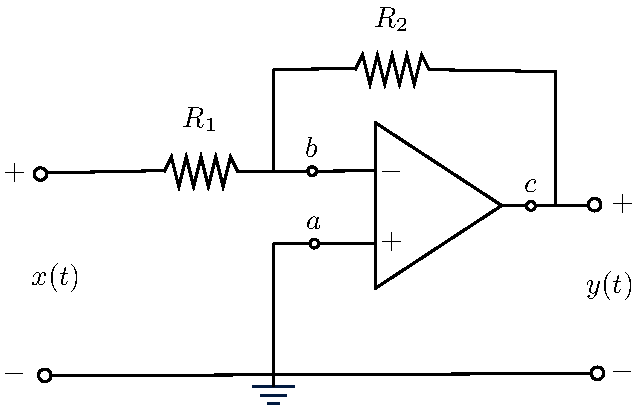
\includegraphics[width=3in]{plots/multiplierbadri1.pdf}
\captionof{figure}{The circuit}
 \label{Fig-Prob2.1a}
}

To simplify the circuit, one has to use the model for the opamp given in Fig.~\ref{Fig-Prob2.1b} which involves the voltage-controlled voltage-source (VCVS) at the output side (indicated in green).  While replacing the operational amplifier with its model, it must be noted that the positive terminal of the operational amplifier is connected to the ground.

{
\centering 
\captionsetup{type=figure}
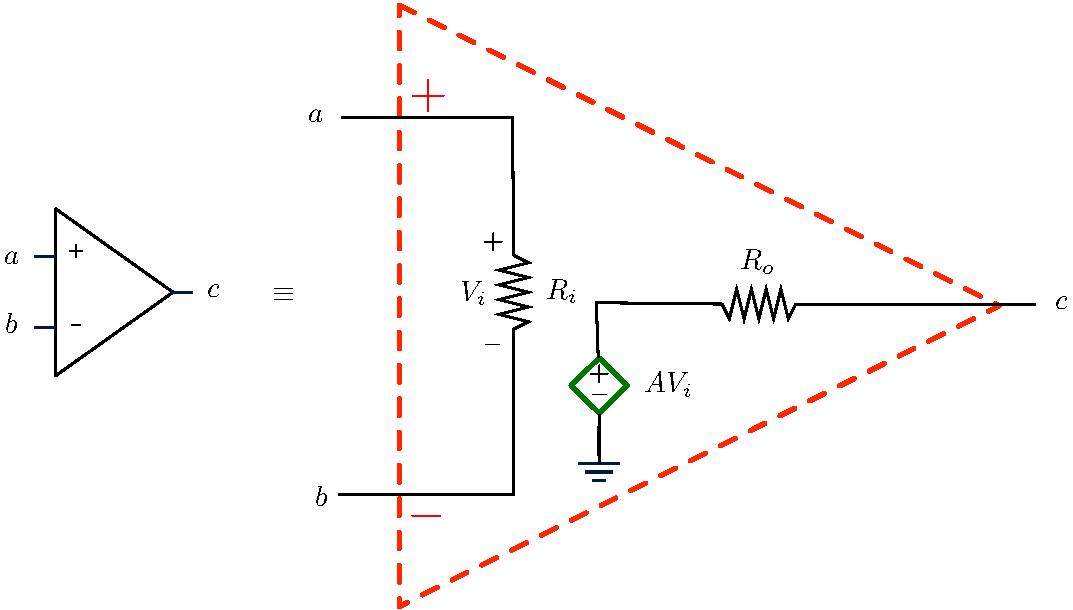
\includegraphics[width=5in]{plots/multiplierbadri2.pdf}
\captionof{figure}{The model for an operational amplifier}
 \label{Fig-Prob2.1b}
}

Upon replacement, we obtain the following equivalent circuit. Again notice that since the positive terminal of the opamp was connected to the ground, the voltage output by the VCVS is $AV_i$ where $V_i$ is the voltage between the ground and the top of the resistance $R_i$, and is measured against the flow of the current $i-i_1$ as is indicated in the figure.

{
\centering 
\captionsetup{type=figure}
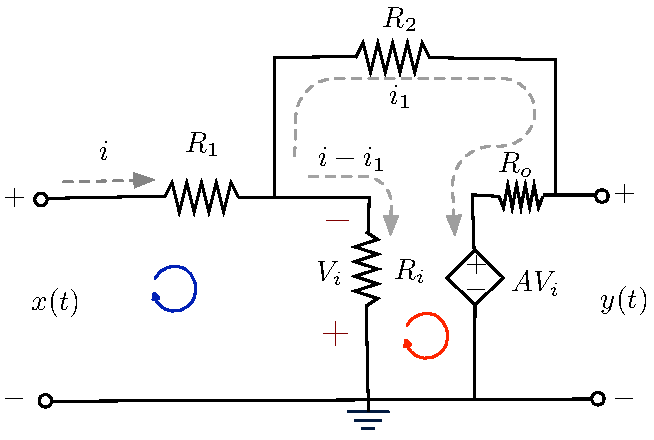
\includegraphics[width=4in]{plots/multiplierbadri3.pdf}
\captionof{figure}{The operational amplifier circuit with the model}
 \label{Fig-Prob2.1c}
}

Applying Kirchoff's law to the outer loop indicated in blue in Fig.~\ref{Fig-Prob2.1c}, we obtain the following equation.
\begin{equation}
x(t) = iR_1+(i-i_1)R_i = i(R_1+R_i) - i_1 R \label{eqn-Prob2.1.1}
\end{equation}
Note that by definition, the voltage $V_i$ that controls the VCVS is the voltage across $R_i$ measured against the indicated direction of the current $i-i_1$, and is given by
\begin{equation}
V_i = -(i-i_1)R_i. \label{eqn-Prob2.1.2}
\end{equation}
Next, writing out the Kirchoff's law for the inner loop indicated in red, we obtain the following.
\begin{align}
0 &= i_1 R_2 + i_2 R_0 + AV_i - (i-i_1) R_i
\end{align}
Substituting $V_i$ in the above equation with the RHS of \eqref{eqn-Prob2.1.2}, we obtain the following.
\begin{align}
0&= i_1 (R_2+R_0) - A(i-i_1)R_i-(i-i_1)R_i\\
&= -i(1+A)R_i+i_1((1+A)R_i+R_0+R_2)\label{eqn-Prob2.1.3}
\end{align}
Combining \eqref{eqn-Prob2.1.3} and \eqref{eqn-Prob2.1.1}, we obtain the following linear system of equations governing the electrical circuit.
\begin{align}
\left[\begin{array}{cc} R_1+R_i &  -R_i\\ -(1+A)R_i & (1+A)R_i+R_0+R_2\end{array}\right]\left[\begin{array}{c} i\\ i_1\end{array}\right] = \left[\begin{array}{c} x(t)\\ 0\end{array}\right]
\end{align}
Solving the above linear system, we identify the current in the different branches to be
\begin{align}
\left[\begin{array}{c} i\\ i_1\end{array}\right] = x(t)\left[\begin{array}{c} \frac{ (1+A)R_i+R_0+R_2}{(1+A) R_iR_1+R_0R_1+R_2R_1+R_0R_i+R_2R_i}\\ \frac{(1+A)R_i}{(1+A) R_iR_1+R_0R_1+R_2R_1+R_0R_i+R_2R_i}\end{array}\right].\label{eqn-Prob2.1.4}
\end{align}
Lastly, notice that
\begin{align}
y(t) &= i_1 R_0 + A V_i \\
 & = i_1 R_0 - (i-i_1)R_i.
\end{align}
Substituting the solutions for $i$ and $i_1$ in terms of $x(t)$, we obtain the following.
\begin{align}
y(t)= \left( \frac{R_iR_0 - R_2R_iA}{(1+A) R_iR_1+R_0R_1+R_2R_1+R_0R_i+R_2R_i} \right)x(t)
\end{align}


\end{solution}

\end{excersizelist}

%%% Local Variables: 
%%% mode: latex
%%% TeX-master: "main.tex"
%%% End: 
